\documentclass[11pt]{article}
\usepackage[colorlinks=true, allcolors=blue]{hyperref}
\usepackage[english]{babel}
\usepackage[numbers]{natbib}
\usepackage{url}
\usepackage[utf8x]{inputenc}
\usepackage{amsmath}
\usepackage{graphicx}
\usepackage{parskip}
\usepackage{fancyhdr}
\usepackage{vmargin}
\usepackage{tikz}
\usepackage{pgfplots} 
\usepackage{minted}
\usepackage{placeins}
\usepackage{tikz}
\usepackage[compatibility,siunitx,  americanvoltages, americancurrents, europeanresistors, europeaninductors, americanports,%
straightlabels, fetbodydiode, straightvoltages]{circuitikz}
\usepackage{amssymb}





\usepackage[compatibility,siunitx,  americanvoltages, americancurrents, europeanresistors, europeaninductors, americanports,%
  straightlabels, fetbodydiode, straightvoltages]{circuitikz}

\usepackage{tikz,amsmath, amssymb,bm,color,pgfkeys,siunitx,ifthen,ulem}
\usepackage{pgfplots}

%\pgfplotsset{compat=1.14}
\usetikzlibrary{shapes,arrows}
%\usepackage{agaramondc}					% Adobe Garamond, custom shape
%\renewcommand{\shapedefault}{rtl} % rtl: roman tabular lining

\makeatletter

%% bandstop filter (adapted from highpass)
\pgfcircdeclarebipole{}{\ctikzvalof{bipoles/highpass/width}}{*bandstop}{\ctikzvalof{bipoles/highpass/width}}{\ctikzvalof{bipoles/highpass/width}}{
	\pgf@circ@res@step = \ctikzvalof{bipoles/highpass/width}\pgf@circ@Rlen
	\divide \pgf@circ@res@step by 2
	
	\pgfpathmoveto{\pgfpoint{\pgf@circ@res@left}{\pgf@circ@res@zero}}
	\pgf@circ@res@other = \pgf@circ@res@left
	\advance\pgf@circ@res@other by \pgf@circ@res@step 
	
	\ifpgf@circuit@dashed
	\pgfsetdash{{0.1cm}{0.1cm}}{0cm} 
	\fi	
	
	% draw outer box
	\pgfsetlinewidth{\pgfkeysvalueof{/tikz/circuitikz/bipoles/thickness}\pgfstartlinewidth}
	\pgfpathrectanglecorners{\pgfpoint{\pgf@circ@res@left}{\pgf@circ@res@up}}{\pgfpoint{\pgf@circ@res@right}{\pgf@circ@res@down}}
	\pgfusepath{draw}
	
	\ifpgf@circuit@inputarrow
	{
		\advance \pgf@circ@res@left by -.5\pgfkeysvalueof{/tikz/circuitikz/bipoles/thickness}\pgfstartlinewidth
		\pgftransformshift{\pgfpoint{\pgf@circ@res@left}{0pt}}
		\pgfnode{inputarrow}{tip}{}{pgf@inputarrow}{\pgfusepath{fill}}
	}
	\fi
	
	% rotate inner symbol
	\def\pgfcircmathresult{\expandafter\pgf@circ@stripdecimals\pgf@circ@direction\pgf@nil}
	\ifnum \pgfcircmathresult > 45 \ifnum \pgfcircmathresult < 135
	\pgftransformrotate{270}
	\fi\fi
	\ifnum \pgfcircmathresult > 134 \ifnum \pgfcircmathresult < 225  % 134 degree, because >= 135 is not possible
	\pgftransformrotate{180}
	\fi\fi
	\ifnum \pgfcircmathresult > 224 \ifnum \pgfcircmathresult < 315
	\pgftransformrotate{90}
	\fi\fi
	
	% draw inner symbol
	\pgfsetdash{}{0pt}	% always draw solid line for inner symbol
	\pgfsetarrows{-} %never draw arrows
	\pgfsetlinewidth{\pgfstartlinewidth}
	\pgfpathmoveto{\pgfpoint{-0.5\pgf@circ@res@step}{0.5\pgf@circ@res@step}}
	\pgfpathsine{\pgfpoint{.25\pgf@circ@res@step}{.25\pgf@circ@res@step}}
	\pgfpathcosine{\pgfpoint{.25\pgf@circ@res@step}{-.25\pgf@circ@res@step}}
	\pgfpathsine{\pgfpoint{.25\pgf@circ@res@step}{-.25\pgf@circ@res@step}}
	\pgfpathcosine{\pgfpoint{.25\pgf@circ@res@step}{.25\pgf@circ@res@step}}
	\pgfusepath{draw}
	
	\pgfpathmoveto{\pgfpoint{-0.5\pgf@circ@res@step}{0}}
	\pgfpathsine{\pgfpoint{.25\pgf@circ@res@step}{.25\pgf@circ@res@step}}
	\pgfpathcosine{\pgfpoint{.25\pgf@circ@res@step}{-.25\pgf@circ@res@step}}
	\pgfpathsine{\pgfpoint{.25\pgf@circ@res@step}{-.25\pgf@circ@res@step}}
	\pgfpathcosine{\pgfpoint{.25\pgf@circ@res@step}{.25\pgf@circ@res@step}}
	\pgfusepath{draw}
	\pgfpathmoveto{\pgfpoint{-0.15\pgf@circ@res@step}{-0.15\pgf@circ@res@step}}
	\pgfpathlineto{\pgfpoint{0.15\pgf@circ@res@step}{0.15\pgf@circ@res@step}}
	\pgfusepath{draw}
	
	\pgfpathmoveto{\pgfpoint{-0.5\pgf@circ@res@step}{-0.5\pgf@circ@res@step}}
	\pgfpathsine{\pgfpoint{.25\pgf@circ@res@step}{.25\pgf@circ@res@step}}
	\pgfpathcosine{\pgfpoint{.25\pgf@circ@res@step}{-.25\pgf@circ@res@step}}
	\pgfpathsine{\pgfpoint{.25\pgf@circ@res@step}{-.25\pgf@circ@res@step}}
	\pgfpathcosine{\pgfpoint{.25\pgf@circ@res@step}{.25\pgf@circ@res@step}}
	\pgfusepath{draw}
	%	\pgfpathmoveto{\pgfpoint{-0.15\pgf@circ@res@step}{-0.65\pgf@circ@res@step}}
	%	\pgfpathlineto{\pgfpoint{0.15\pgf@circ@res@step}{-0.35\pgf@circ@res@step}}
	%	\pgfusepath{draw}
}

\tikzset{
	*bandstop/.style={\circuitikzbasekey, /tikz/to path=\pgf@circ@*bandstop@path},
}
\def\pgf@circ@*bandstop@path#1{\pgf@circ@bipole@path{*bandstop}{#1}}




\makeatother


\usetikzlibrary{backgrounds,calc,positioning}

\usetikzlibrary{circuits.ee.IEC}
\usetikzlibrary{arrows}


% sym32a style

\ctikzset{tripoles/mos style/arrows}
\ctikzset{
	/tikz/circuitikz/quadpoles/coupler/width=1,%1.3
	/tikz/circuitikz/quadpoles/coupler/height=0.952,%1.3
	/tikz/circuitikz/quadpoles/coupler2/width=1,%1.3
	/tikz/circuitikz/quadpoles/coupler2/height=0.952,%1.3
	/tikz/circuitikz/quadpoles/transformer/width=1.425,%1.5
	/tikz/circuitikz/quadpoles/transformer/height=1.425,%1.5
	/tikz/circuitikz/quadpoles/transformer core/width=1.425,%1.5
	/tikz/circuitikz/quadpoles/transformer core/height=1.425,%1.5
	/tikz/circuitikz/quadpoles/gyrator/width=1.425,%1.5
	/tikz/circuitikz/quadpoles/gyrator/height=1.425,%1.5
	%/tikz/circuitikz/monopoles/tlinestub/width=0.1875,%0.25 no effect!
	/tikz/circuitikz/tripoles/american and port/height=0.95,%.8
	/tikz/circuitikz/tripoles/american nand port/height=0.95,%.8
	/tikz/circuitikz/tripoles/american or port/height=0.95,%.8
	/tikz/circuitikz/tripoles/american nor port/height=0.95,%.8
	/tikz/circuitikz/tripoles/american xor port/height=0.95,%.8
	/tikz/circuitikz/tripoles/american xnor port/height=0.95,%.8
	/tikz/circuitikz/bipoles/tline/height=0.4,%0.3
%	/tikz/circuitikz/bipoles/tline/width=1.2,%0.8
	/tikz/circuitikz/bipoles/diode/height=0.375,%
	/tikz/circuitikz/bipoles/diode/width=0.375,%
	/tikz/circuitikz/bipoles/varcap/height=0.375,%
	/tikz/circuitikz/bipoles/varcap/width=0.375,%
	/tikz/circuitikz/tripoles/triac/height=1.05,%
	/tikz/circuitikz/tripoles/triac/width=0.952,%
	/tikz/circuitikz/tripoles/thyristor/height=1.05,%
	/tikz/circuitikz/tripoles/thyristor/width=0.952,%
	/tikz/circuitikz/tripoles/op amp/height=0.952,%
	/tikz/circuitikz/tripoles/op amp/width=1.2,%
	/tikz/circuitikz/tripoles/op amp/font=\footnotesize,
	/tikz/circuitikz/tripoles/gm amp/height=0.952,% 1.7
	/tikz/circuitikz/tripoles/gm amp/width=1.2,% 1.4
	%	/tikz/circuitikz/tripoles/gm amp/font=\footnotesize,
	/tikz/circuitikz/tripoles/plain amp/height=0.952,% 1.7
	/tikz/circuitikz/tripoles/plain amp/width=1.2,% 1.4
	/tikz/circuitikz/bipoles/resistor/voltage/straight label distance/.initial=.8,
	/tikz/circuitikz/bipoles/generic/voltage/straight label distance/.initial=.8,
	/tikz/circuitikz/bipoles/inductor/voltage/straight label distance/.initial=.8,
	/tikz/circuitikz/bipoles/fullgeneric/voltage/straight label distance/.initial=.8,
	/tikz/circuitikz/bipoles/capacitor/voltage/straight label distance/.initial=1.0,
	/tikz/circuitikz/bipoles/thickness=1.6,
}
\ctikzset{v/.append style={/tikz/european voltages}}

\definecolor{netlabelcolor}{rgb}{0, 0, 0.25}
\definecolor{lttotitextcolor}{rgb}{0, 0.4, 0.25}
\definecolor{lttotidrawcolor}{rgb}{0.6, 0.6, 0.6}
\definecolor{netcolor}{rgb}{0, 0, 0.5}

\pgfkeys{/lt2ti/netlabel/font/.initial= \small}
\pgfkeys{/lt2ti/text/font/.initial= \small}

\pgfkeys{/lt2ti/Net/.style= {netcolor}}
\tikzstyle{dashdotdotted}=[dash pattern=on 3pt off 2pt on \the\pgflinewidth off 2pt on \the\pgflinewidth off 2pt]

\pgfkeys{/lt2ti/VArrow/.style= {->,>=latex}}
\pgfkeys{/lt2ti/SArrow/.style= {->,>=angle 90}}
%%%%%%%%%%%%%%%%%%%%%%%%%%%%%%%%%%%%%%%%%%%%%%%%%%%%%%%%%%%%%%%%%%%%%%%%%%%%%%%


\def\WSPath{/home/g/Uni code/Electronic Processing and Communications (EEEE2044 UNUK)/EEEE2044 Coursework 1 - Digital Electronics/}
\def\LTSpicePath{/home/g/.var/app/com.usebottles.bottles/data/bottles/bottles/UNI/drive_c/Program Files/LTC/LTspiceXVII/lib/sym}
\def\LT2Tikzscript{tools/lt2circuitikz-master/lt2ti.py}

\newcommand{\LTSpice}[1]{\input{|python3 \LT2Tikzscript '\WSPath#1'}}

%%%%%%%%%%%%%%%%%%%%%%%%%%%%%%%%%%%%%%%%%%%%%%%%%%%%%%%%%%%%%%%%%%%%%%%%%%%%%%%
\title{Coursework 1 (Fourier
Transforms)}								
\author{George Downing}								                        
\date{December 20, 2022}					

\graphicspath{{images/}}
\setmarginsrb{3 cm}{2.5 cm}{3 cm}{2.5 cm}{1 cm}{1.5 cm}{1 cm}{1.5 cm}

\usetikzlibrary{angles,quotes} 
\usetikzlibrary{arrows.meta}
\usetikzlibrary{calc}
\ctikzset{tripoles/mos style/arrows} 		
\usetikzlibrary{matrix,calc}				            

\makeatletter
\let\thetitle\@title
\let\theauthor\@author
\let\thedate\@date
\makeatother

\pagestyle{fancy}
\fancyhf{}
\rhead{\theauthor}
\lhead{\thetitle}
\cfoot{\thepage}

\newcommand{\Q}{Q1} 

\newenvironment{conditions}[1][where:]
  {#1 \begin{tabular}[t]{>{$}l<{$} @{${}={}$} l}}
  {\end{tabular}\\[\belowdisplayskip]}
\begin{document}

%%%%%%%%%%%%%%%%%%%%%%%%%%%%%%%%%%%%%%%%%%%%%%%%%%%%%%%%%%%%%%%%%%%%%%%%%%%%%%%%%%%%%%%%%
                                    % Title Page
%%%%%%%%%%%%%%%%%%%%%%%%%%%%%%%%%%%%%%%%%%%%%%%%%%%%%%%%%%%%%%%%%%%%%%%%%%%%%%%%%%%%%%%%%

\begin{titlepage}
    \centering
    %\vspace*{0.5 cm}
    
\includegraphics[scale = 0.4]{Config/uon.png}\\[1.0 cm]	% University Logo

    
    \textsc{\Large Department of Electrical and Electronic Engineering
    Faculty of Engineering}\\[1.5 cm]	% University Name
    \textsc{\large Modelling: Methods and Tools}\\[0.5 cm]				% Course Code
    \textsc{\large (EEEE2055 UNUK) (FYR1 22-23)}\\[0.5 cm]				% Course Name

    \rule{\linewidth}{0.2 mm} \\[0.4 cm]
    { \huge \bfseries \thetitle}\\
    \rule{\linewidth}{0.2 mm} \\[1.5 cm]

    \begin{minipage}{0.4\textwidth}
        \begin{flushleft} \large
            \emph{Author:}\\
            \theauthor
        \end{flushleft}
    \end{minipage}~
    \begin{minipage}{0.4\textwidth}
        \begin{flushright} \large
            \emph{Student Number:} \\
            20273662									% Your Student Number
        \end{flushright}
    \end{minipage}\\[1.5 cm]

    {\large \thedate}\\[0 cm]

    \vfill

\end{titlepage}
\pagebreak

%%%%%%%%%%%%%%%%%%%%%%%%%%%%%%%%%%%%%%%%%%%%%%%%%%%%%%%%%%%%%%%%%%%%%%%%%%%%%%%%%%%%%%%%%
                                    % Table of Contents
%%%%%%%%%%%%%%%%%%%%%%%%%%%%%%%%%%%%%%%%%%%%%%%%%%%%%%%%%%%%%%%%%%%%%%%%%%%%%%%%%%%%%%%%%

\tableofcontents
\pagebreak



%%%%%%%%%%%%%%%%%%%%%%%%%%%%%%%%%%%%%%%%%%%%%%%%%%%%%%%%%%%%%%%%%%%%%%%%%%%%%%%%%%%%%%%%%
                            % Fourier Transform of a Signal
%%%%%%%%%%%%%%%%%%%%%%%%%%%%%%%%%%%%%%%%%%%%%%%%%%%%%%%%%%%%%%%%%%%%%%%%%%%%%%%%%%%%%%%%%

\section{Fourier Transform of a Signal}\label{sec:fourier_transform_of_a_signal}

\subsection{Fourier Transform derivation}\label{subsec:fourier_transform_derivation}
% Derive the Fourier Transform of the S2(t) (see Figure 1 [Report: derivation of Fourier Transform including
% some comments to explain each step]
\begin{figure}[ht!]
	\centering
	% This file was created by matlab2tikz.
%
%The latest updates can be retrieved from
%  http://www.mathworks.com/matlabcentral/fileexchange/22022-matlab2tikz-matlab2tikz
%where you can also make suggestions and rate matlab2tikz.
%
\definecolor{mycolor1}{rgb}{0.00000,0.44706,0.74118}%
%
\begin{tikzpicture}

\begin{axis}[%
width=4.568in,
height=3.603in,
at={(0.766in,0.486in)},
scale only axis,
xmin=0,
xmax=0.003,
xlabel style={font=\color{white!15!black}},
xlabel={time[s]},
ymin=-0.1,
ymax=1.1,
ylabel style={font=\color{white!15!black}},
ylabel={[arb]},
axis background/.style={fill=white}
]
\addplot [color=mycolor1, line width=1.1pt, forget plot]
  table[row sep=crcr]{%
0	0\\
0.001	0\\
0.00199969996999705	0.999699969997\\
0.00200090009000897	0\\
0.003	0\\
};
\end{axis}
\end{tikzpicture}%
	\caption{$S_{2}(t)$}\label{fig:S2}
\end{figure}\FloatBarrier

\begin{figure}[ht!]
	\centering
	% This file was created by matlab2tikz.
%
%The latest updates can be retrieved from
%  http://www.mathworks.com/matlabcentral/fileexchange/22022-matlab2tikz-matlab2tikz
%where you can also make suggestions and rate matlab2tikz.
%
\definecolor{mycolor1}{rgb}{0.00000,0.44706,0.74118}%
%
\begin{tikzpicture}

\begin{axis}[%
width=4.568in,
height=3.603in,
at={(0.766in,0.486in)},
scale only axis,
xmin=0,
xmax=0.003,
xlabel style={font=\color{white!15!black}},
xlabel={time[s]},
ymin=-300,
ymax=1100,
ylabel style={font=\color{white!15!black}},
ylabel={[arb]},
axis background/.style={fill=white},
axis x line*=bottom,
axis y line*=left
]
\addplot [color=mycolor1, line width=1.1pt, forget plot]
  table[row sep=crcr]{%
0	0\\
0.000999699969952417	0\\
0.00100090009004816	1000\\
0.00199969997004246	1000\\
0.00200090009002452	0\\
0.00300000000004275	0\\
};
\addplot[ycomb, color=mycolor1, line width=1.1pt, mark=triangle, mark options={solid, rotate=180, mycolor1}, forget plot] table[row sep=crcr] {%
0.002	-200\\
};
\addplot[forget plot, color=white!15!black, line width=1.1pt] table[row sep=crcr] {%
0	0\\
0.003	0\\
};
\end{axis}
\end{tikzpicture}%
	\caption{$\frac{dS_{2}\left(t\right)}{dt}$}\label{fig:dS2}
\end{figure}\FloatBarrier



Figure \ref{fig:S2} shows the triangular pulse $S_{2}(t)$ and Figure \ref{fig:dS2} shows the derivative of $S_{2}(t)$. where the gradient of the triangle represents a rise of 1 in 1ms.

To calculate the fourier transform of the signal we can split the signal allowing us to differentiate the the different components to create delta functions. The first derivative of $S_{2}(t)$ is shown in \eqref{eq:first_derivative_of_S2}. This signal consists of a rectangular pulse with a width of 1ms and a height of 1000 can be differentiated again to form two unit impulses. Also there is unit impulse at 0.002ms.

The second derivative of $S_{2}(t)$ as a summation of delta functions is shown in \eqref{eq:second_derivative_of_S2}. 

\begin{equation}
	\begin{split}
		\frac{d^{2}S_{2}\left(t\right)}{dt^{2}} &= \frac{d}{dt}\left[\frac{dS_{2}\left(t\right)}{dt}\right]\\
		&= \left(\frac{1}{m}\delta\left(t - m\right) - \frac{1}{m}\delta\left(t - 2m\right)\right) + \frac{d}{dt}\left[\delta\left(t - 2m\right)\right]\\
		&= 1000\delta\left(t - 0.001\right) - 1000\delta\left(t - 0.002\right) + \frac{d}{dt}\left[\delta\left(t - 0.002\right)\right]
	\end{split}
	\label{eq:second_derivative_of_S2}
\end{equation}

In order to calculate the fourier transform of the Signal $S_{2}(t)$ we can use the derivative theorem. The derivative theorem states that the fourier transform of the derivative of a signal is the fourier transform of the signal divided by the frequency. Application of derivative theorem is shown in \eqref{eq:derivative_theorem}. Where the first line is the derivative theorem and the second line is the application of the derivative theorem to the second derivative of $S_{2}(t)$.

\begin{equation}
	\begin{split}
		\left(j\omega\right)^{2} \mathcal{F}\left\{S\left(t\right)\right\} =& \mathcal{F}\left\{\frac{d^{2}S_{2}\left(t\right)}{dt^{2}}\right\}\\
		\therefore \widetilde{S} \left\{\omega\right\} =& \frac{1}{\left(j\omega\right)^{2}} \cdot \mathcal{F}\left\{1000\delta\left(t - 0.001\right) - 1000\delta\left(t - 0.002\right)\right\}\\
		&+ \frac{1}{\left(j\omega\right)} \cdot \mathcal{F}\delta\left(t - 0.002\right)\\
	\end{split}
	\label{eq:derivative_theorem}
\end{equation}

The Fourier transform is evaluated using integration as shown in \eqref{eq:fourier_transform_of_S2}. 

\begin{equation}
	\begin{split}
		\widetilde{S} \left\{\omega\right\}
		=& \frac{1000}{\left(j\omega\right)^{2}} \cdot \int_{-\infty}^{\infty}\delta\left(t - 0.001\right)e^{-j\omega t}dt\\
		&  + \frac{-1000}{\left(j\omega\right)^{2}}\cdot  \int_{-\infty}^{\infty}\delta\left(t - 0.002\right)e^{-j\omega t}dt\\
		&  + \frac{-1}{j\omega} \cdot \int_{-\infty}^{\infty}\delta\left(t - 0.002\right)e^{-j\omega t}dt\\
	\end{split}
	\label{eq:fourier_transform_of_S2}
\end{equation}

The equation given in \eqref{eq:fourier_transform_of_S2} is then evaluated, using the properties of the delta function, to give the following equation \eqref{eq:fourier_transform_of_S2_evaluated}. 

\begin{equation}
	\begin{split}
		\widetilde{S} \left\{\omega\right\} =& \frac{-1000} {\omega^2} \cdot e^{-j\omega 0.001}\\
		& + \frac{1000} {\omega^2}  \cdot e^{-j\omega 0.002m}\\
		& + \frac{-1} {j\omega}  \cdot e^{-j\omega 0.002m}\\
		=& \frac{1}{\left(j \omega\right)^{2} m}\left[e^{-j\omega 0.001m} - e^{-j\omega 0.002m}\right] - \frac{1}{\left(j \omega\right)}\left[e^{-j\omega 0.001m} - e^{-j\omega 0.002m}\right]\\
		\label{eq:fourier_transform_of_S2_evaluated}
	\end{split}
\end{equation}

The equation given in \eqref{eq:fourier_transform_of_S2_evaluated} is then simplified to give the following equation \eqref{eq:fourier_transform_of_S2_simplified}.

\begin{equation}
	\widetilde{S} \left\{\omega\right\} = \frac{je^{-\frac{j\omega}{500}}}{\omega}+\frac{1000e^{-\frac{j\omega}{500}}-1000e^{-\frac{j\omega}{1000}}}{\omega^2}\label{eq:fourier_transform_of_S2_simplified}
\end{equation}

Converting the equation into polar form to avoid imaginary exponentials gives the following equation \eqref{eq:fourier_transform_of_S2_polar}.

\begin{equation}
		\widetilde{S} \left\{\omega\right\} = \frac{t\sin \left(\frac\omega{500}\right)-2000\sin \left(\frac\omega{2000}\right)\sin \left(\frac{3t}{2000}\right)}{t^2}+j\frac{t\cos \left(\frac\omega{500}\right)-2000\sin \left(\frac\omega{2000}\right)\cos \left(\frac\omega{2000}-\frac\omega{500}\right)}{t^2}
	\label{eq:fourier_transform_of_S2_polar}
\end{equation}

\begin{figure}[ht!]
	\centering
	% This file was created by matlab2tikz.
%
%The latest updates can be retrieved from
%  http://www.mathworks.com/matlabcentral/fileexchange/22022-matlab2tikz-matlab2tikz
%where you can also make suggestions and rate matlab2tikz.
%
\definecolor{mycolor1}{rgb}{0.00000,0.44700,0.74100}%
\definecolor{mycolor2}{rgb}{0.85000,0.32500,0.09800}%
%
\begin{tikzpicture}

\begin{axis}[%
width=4.568in,
height=3.603in,
at={(0.766in,0.486in)},
scale only axis,
xmin=0,
xmax=35000,
ymin=-55,
ymax=-10,
axis background/.style={fill=white},
axis x line*=bottom,
axis y line*=left
]
\addplot [color=mycolor1, forget plot]
  table[row sep=crcr]{%
159.200000000001	-12.8021258830777\\
201.022358800805	-12.9465751484349\\
242.005337891715	-13.1212883452026\\
283.72265444247	-13.3332358744083\\
323.930299018695	-13.5705042116933\\
364.000703126992	-13.8396507787256\\
404.714037925685	-14.147062347176\\
445.235423485981	-14.4875609173469\\
484.648136160638	-14.8523464937789\\
524.760432606057	-15.258174392533\\
565.188496173265	-15.7029843393466\\
605.512682058208	-16.1828391500931\\
645.283961998372	-16.691717398553\\
684.031649426361	-17.2214104244231\\
725.106038538317	-17.8188814910427\\
764.582836879039	-18.4267696371062\\
806.208862400894	-19.1010628747354\\
850.101125035555	-19.8445420997159\\
905.93746145433	-20.826204748395\\
1018.00255782626	-22.8078950220188\\
1050.90312391032	-23.3531271791981\\
1079.13106439784	-23.7920454560044\\
1108.11722570137	-24.2067208403678\\
1131.86574162414	-24.5141323932112\\
1156.12322175706	-24.7943701115873\\
1180.9005739214	-25.042909308464\\
1206.20893970845	-25.2562736236214\\
1232.0596994895	-25.4324635211851\\
1258.46447753327	-25.5712651895192\\
1285.43514723297	-25.6743720696504\\
1312.98383644536	-25.7452909079002\\
1348.25143509741	-25.7964546264957\\
1391.82523075963	-25.819152432854\\
1531.17964282111	-25.855918073612\\
1572.30812255426	-25.9110220710063\\
1614.54133996669	-26.0034128961306\\
1649.14323932431	-26.1088295425252\\
1684.4867062154	-26.245274455061\\
1720.58763347868	-26.4147882955658\\
1757.46225455889	-26.6186231586544\\
1795.12715080634	-26.8571046431935\\
1833.5992589331	-27.1294228887709\\
1882.85092598167	-27.5138384038728\\
1943.70230679642	-28.0279602308656\\
2060.41676720788	-29.029655251994\\
2104.57440619107	-29.3716873391713\\
2138.31258271326	-29.6055859071785\\
2172.59161184284	-29.8133071154807\\
2207.42016392223	-29.9899491389806\\
2242.80704828705	-30.1324208240985\\
2278.76121549431	-30.2399470258097\\
2315.29175958631	-30.3142988561412\\
2352.40792039084	-30.3596857844132\\
2402.82334184491	-30.3861247633577\\
2587.93923239034	-30.4331321377394\\
2643.40242224255	-30.5069816501455\\
2685.77848520257	-30.5952880669101\\
2728.83387367764	-30.7152447615772\\
2772.57947785254	-30.8683240304927\\
2817.02636249127	-31.054329630384\\
2862.18576973569	-31.2711791308975\\
2923.52644990015	-31.6006547605175\\
3099.07689860088	-32.587035544595\\
3148.75782371013	-32.8206777882842\\
3199.23517769175	-33.0157759529102\\
3233.33550402625	-33.1203451024194\\
3285.1687125217	-33.2366278060945\\
3337.8328528829	-33.3067799924465\\
3391.34124567759	-33.33943413421\\
3482.43487426978	-33.3483881137545\\
3575.97533689279	-33.365409842474\\
3633.30136290554	-33.408202845123\\
3691.54637547407	-33.489101279898\\
3750.72510676018	-33.6147375500805\\
3810.85252509512	-33.7871779578963\\
3871.9438387657	-34.0033853825698\\
3954.92505932094	-34.3439830350471\\
4082.74327772453	-34.8873767374971\\
4148.19323900575	-35.1269514506057\\
4192.40841397478	-35.2604170226805\\
4237.09487405153	-35.3679029029081\\
4282.25764261663	-35.4476810506749\\
4327.9017965944	-35.5006991844311\\
4397.28186429581	-35.5385398763174\\
4515.39571127947	-35.5462266619143\\
4587.78147113976	-35.5609671072998\\
4661.32763831884	-35.6127032875484\\
4711.01226129595	-35.6761325545704\\
4761.2264676776	-35.7659619763581\\
4811.97590224009	-35.8826631725024\\
4889.11610309625	-36.1036150215841\\
4993.89676071046	-36.4564491116143\\
5100.92301568391	-36.8136279556093\\
5155.29324162258	-36.9685639081363\\
5210.24299433699	-37.0959063311784\\
5265.77845094484	-37.1905257469225\\
5321.90585440505	-37.2517561891291\\
5378.63151421967	-37.2837282967957\\
5464.85570232191	-37.2957821405471\\
5581.97527203176	-37.3053491157407\\
5641.4729856399	-37.3329716173976\\
5701.60487939971	-37.3875169068597\\
5762.37771297372	-37.4738437908418\\
5823.79831807498	-37.5929958747729\\
5885.87359923516	-37.7418911385503\\
5980.22932355363	-38.0040443158359\\
6108.39407726217	-38.3608808986974\\
6173.50283602641	-38.5102509107928\\
6239.30558250891	-38.6247230126937\\
6305.809713855	-38.6996564427427\\
6373.0227060555	-38.7380716636071\\
6475.18785849882	-38.7509986378936\\
6613.96027209715	-38.7680583677175\\
6684.45781013831	-38.8107910451399\\
6755.70677435463	-38.8896895049511\\
6827.71517412222	-39.007405325021\\
6900.4911041883	-39.1597745198596\\
7161.37006348581	-39.7643146558257\\
7237.70238749558	-39.8833103552315\\
7314.84833007792	-39.9570237256667\\
7392.81656351148	-39.989800712854\\
7672.30830725065	-40.0386943683006\\
7754.08667066717	-40.1131051282209\\
7836.73670144314	-40.2321722479646\\
7920.26769059338	-40.3899118020272\\
8133.01122511005	-40.8309328401738\\
8219.70017464159	-40.9630549695175\\
8307.31313297663	-41.0450268992136\\
8395.85994903215	-41.0797234221645\\
8667.20361409661	-41.1189364314814\\
8759.58646663251	-41.1928411667977\\
8852.95401871194	-41.3170563204803\\
8947.31676614844	-41.4821820849938\\
9139.07039090813	-41.8337837117797\\
9236.48282401	-41.9600076856877\\
9334.93356644935	-42.0297714314147\\
9434.43368546108	-42.051614234002\\
9636.62691322149	-42.0696866113394\\
9739.3427513056	-42.1296567671889\\
9843.15342718805	-42.2455303381394\\
9948.07061063497	-42.4087447431593\\
10107.5469215363	-42.6776307384534\\
10215.2822486761	-42.8177006984879\\
10324.1659158438	-42.897228314323\\
10434.2101630804	-42.9218406397995\\
10601.4797180631	-42.9295543192093\\
10714.4798252561	-42.9743148574162\\
10828.6843892386	-43.079148596622\\
10944.1062481945	-43.2386754188228\\
11119.5498853465	-43.5058627911567\\
11238.0720504024	-43.6371855288271\\
11357.8575313079	-43.7012899971778\\
11478.9197936195	-43.7137880106711\\
11601.2724464221	-43.7196132451609\\
11724.9292438583	-43.7665480803771\\
11849.9040866747	-43.8795302806939\\
11976.2110237845	-44.0475099370997\\
12103.864253847	-44.2268414557329\\
12232.8781268635	-44.3635454823889\\
12297.8998306342	-44.4048944835631\\
12428.9819093691	-44.4372165817731\\
12628.2294077782	-44.4486717318941\\
12695.3525314769	-44.4712673190552\\
12762.832436288	-44.511581227518\\
12898.8701849552	-44.6463835765353\\
13175.3111759155	-44.9887235311362\\
13245.3422161566	-45.0462912254152\\
13315.745494027	-45.0834293127664\\
13457.6766874259	-45.1071941170921\\
13601.1207111555	-45.1121276412159\\
13673.4150667976	-45.1289560112491\\
13746.0936903224	-45.1637822105949\\
13819.1586242379	-45.2188580693401\\
13966.4556476143	-45.3793637035742\\
14115.322695164	-45.5578081636522\\
14190.3502006614	-45.6305945606073\\
14265.7765016169	-45.6832005651813\\
14341.6037177575	-45.7139978149025\\
14494.469430896	-45.72844545505\\
14648.9645243126	-45.7413430394663\\
14726.8285087297	-45.7701989062225\\
14805.1063654079	-45.8205085968002\\
14962.9125067	-45.9773496169291\\
15122.4006877975	-46.155126199028\\
15202.7811385488	-46.225618684035\\
15283.5888373936	-46.2739638328094\\
15364.8260552938	-46.2994485533491\\
15694.1159605145	-46.3331627452208\\
15777.5352628524	-46.3748925227883\\
15861.3979657628	-46.4395152964207\\
16201.3301077876	-46.7725346417246\\
16287.4454173684	-46.8206650250504\\
16374.0184576723	-46.8446542012352\\
16724.9367802492	-46.8866106222486\\
16813.8352286463	-46.9375966048174\\
16993.0522090763	-47.10014465516\\
17174.179445295	-47.2688167888045\\
17265.465763757	-47.3241419789447\\
17357.2372985268	-47.3533800891091\\
17729.2273883825	-47.3974184978579\\
17823.4639661834	-47.4502080883503\\
18013.4424778902	-47.6166786892754\\
18109.1897508165	-47.7052564701589\\
18205.4459514664	-47.7771679905454\\
18302.2137849552	-47.8228165273467\\
18497.2952428808	-47.8453277248736\\
18694.4560544667	-47.8660325249293\\
18793.8231348154	-47.9097038730069\\
18893.7183833347	-47.9799537668514\\
19196.6012864539	-48.2325124397357\\
19298.6374311214	-48.2800785225299\\
19401.2159308996	-48.2998861753549\\
19608.0115422829	-48.3062468359713\\
19712.2344655241	-48.3276864423315\\
19817.0113673115	-48.3769666092667\\
20028.2389004769	-48.5433397142442\\
20134.6954680426	-48.6295046749765\\
20241.7178866965	-48.6937583952022\\
20349.3091641202	-48.7277962838089\\
20675.5264661382	-48.7509473651153\\
20785.4235764701	-48.7905917553435\\
20895.9048254877	-48.859848494998\\
21118.6321756283	-49.0366993089374\\
21230.8845361215	-49.1044670366864\\
21343.7335542169	-49.1409353840354\\
21685.8923527732	-49.1663325142363\\
21801.159884579	-49.2094962269803\\
22033.5362574442	-49.3731236913409\\
22150.6516290432	-49.4577350216823\\
22268.3895067212	-49.5163756076763\\
22386.7531992995	-49.5421463776402\\
22625.3713524723	-49.5505464508969\\
22745.6325190207	-49.5779987489113\\
22866.5329125659	-49.6382441802925\\
23233.1035225597	-49.8817873031112\\
23356.5949821532	-49.9164295665396\\
23731.0217176238	-49.9494672888504\\
23857.1597734678	-50.0063845340374\\
24239.6110022709	-50.2479806390984\\
24368.4523746577	-50.2802489603819\\
24628.193260241	-50.2901749860866\\
24759.1000730096	-50.3195787309487\\
24890.7026978277	-50.3844422276889\\
25156.0101971356	-50.5578841677561\\
25289.7225276376	-50.6130528140129\\
25424.1455824233	-50.6322037249774\\
25695.1389958435	-50.6478016719338\\
25831.7169702831	-50.6960811062818\\
26245.8220855268	-50.9344909707943\\
26385.3271186976	-50.9639612444807\\
26666.5656695438	-50.9761971463959\\
26808.3070909464	-51.0171909195378\\
27238.0678037228	-51.2546586414792\\
27382.8469438115	-51.285620630526\\
27674.7179582537	-51.2988665365774\\
27821.8180351413	-51.3427545520026\\
28267.826218685	-51.5753739404645\\
28418.078857808	-51.5982511104994\\
28720.9843052125	-51.6177922158895\\
28873.6456261322	-51.6749826183441\\
29181.4069139499	-51.8448775387369\\
29336.5155299511	-51.8902687839618\\
29649.2105015694	-51.9046386209702\\
29806.8056449424	-51.9428156716131\\
30284.6349236096	-52.1701696542368\\
30770.1242253691	-52.2184977432844\\
30933.6773877255	-52.2890603590058\\
31098.0998880384	-52.3790873768558\\
31263.3963471203	-52.4456486390081\\
31429.5714103447	-52.4681517580175\\
31596.6297477767	-52.4702793197175\\
31764.5760543046	-52.4960841339052\\
};
\addplot [color=mycolor2, only marks, mark=o, mark options={solid, mycolor2}, forget plot]
  table[row sep=crcr]{%
0	-15.563025530344\\
333.333333333332	-13.6238715620311\\
666.666666666668	-16.9750405995255\\
1000	-22.4957227642408\\
1333.33333333333	-25.7724527512401\\
1666.66666666667	-26.1671837232607\\
2000	-28.5163223019699\\
2333.33333333333	-30.3330722950668\\
2666.66666666667	-30.5460102123834\\
3000	-32.0381477860356\\
3333.33333333333	-33.2959208414686\\
3666.66666666667	-33.4435636294438\\
4000	-34.5369221376532\\
4333.33333333333	-35.4988907622574\\
4666.66666666667	-35.6123226309064\\
5000	-36.4751228555433\\
5333.33333333333	-37.253963003197\\
5666.66666666667	-37.3461943500442\\
6000	-38.0587475020875\\
6333.33333333333	-38.7130442570415\\
6666.66666666667	-38.7908069599835\\
7000	-39.3976833690285\\
7333.33333333333	-39.9617809163756\\
7666.66666666667	-40.0290237282788\\
8000	-40.55752222499\\
8333.33333333333	-41.0532790631041\\
8666.66666666667	-41.1125218133566\\
9000	-41.5805727187617\\
9333.33333333333	-42.0227595613651\\
9666.66666666667	-42.0757103113938\\
10000	-42.4957225008875\\
10333.3333333333	-42.8947882623143\\
10666.6666666667	-42.9426592883647\\
11000	-43.3235762029399\\
11333.3333333333	-43.6871841807879\\
11666.6666666667	-43.7308673094885\\
12000	-44.0793474235106\\
12333.3333333333	-44.413284603972\\
12666.6666666667	-44.4534552305631\\
13000	-44.7745895251865\\
13333.3333333333	-45.0833331831236\\
13666.6666666667	-45.1205152744296\\
14000	-45.4182832490187\\
14333.3333333333	-45.7053680263416\\
14666.6666666667	-45.7399761086454\\
15000	-46.0175477063749\\
15333.3333333333	-46.2858135498427\\
15666.6666666667	-46.3181814524687\\
16000	-46.578122129933\\
16333.3333333333	-46.8298843752382\\
16666.6666666667	-46.8602849614654\\
17000	-47.1047009370632\\
17333.3333333333	-47.3418725894262\\
17666.6666666667	-47.3705315117659\\
18000	-47.6011726080469\\
18333.3333333333	-47.8253521759616\\
18666.6666666667	-47.8524584152619\\
19000	-48.0707945289359\\
19333.3333333333	-48.283331541752\\
19666.6666666667	-48.3090448423791\\
20000	-48.5163224325152\\
20333.3333333333	-48.718366482055\\
20666.6666666667	-48.7428231252816\\
21000	-48.9401083966841\\
21333.3333333333	-49.1326468252737\\
21666.6666666667	-49.1559640423984\\
22000	-49.3441761448339\\
22333.3333333333	-49.5280632108334\\
22666.6666666667	-49.5503424832496\\
23000	-49.7302792240298\\
23333.3333333333	-49.9062589383284\\
23666.6666666667	-49.9275888349366\\
24000	-50.0999473814081\\
24333.3333333333	-50.2686718272489\\
24666.6666666667	-50.2891299077528\\
25000	-50.4545226343398\\
25333.3333333333	-50.6165663556421\\
25666.6666666667	-50.636221287783\\
26000	-50.7951894833823\\
26333.3333333333	-50.9510613276216\\
26666.6666666667	-50.9699736977527\\
27000	-51.1229977725525\\
27333.3333333333	-51.2731506889868\\
27666.6666666667	-51.2913746525373\\
28000	-51.4388831370961\\
28333.3333333333	-51.5837219146415\\
28666.6666666667	-51.6013058098542\\
29000	-51.7436824554934\\
29333.3333333333	-51.8835703980003\\
29666.6666666667	-51.9005577006174\\
30000	-52.0381475887189\\
30333.3333333333	-52.1734119706598\\
30666.6666666667	-52.1898418564379\\
31000	-52.3229563855639\\
31333.3333333333	-52.4538930475173\\
31666.6666666667	-52.4698009225795\\
};
\end{axis}
\end{tikzpicture}%
	\caption{$S_2\left(f\right)$}\label{fig:s2f} 
\end{figure}\FloatBarrier 



\subsection{How can an FFT differ from theory}\label{subsec:fourier_transform_of_a_square_wave}
% Use LTSpice to verify your answer and to look for differences between an FFT and the theoretical Fourier
% Transform.
% As a hint, your LTSpice and calculated plots should be very similar at lower frequencies but there will be
% some small differences at higher frequencies. If your plot looks completely different then something isn’t correct.
% You should try to compare your result from the derivation and the LTSpice result on the same plot (export
% data from LTSpice to Excel, etc). Also think carefully about:
% ˆ The frequency range used - you need to make this is wide enough to see any/all differences (i.e. starts at
% a low enough frequency and finishes at a high enough frequency)
% ˆ The axis scales used, see tutorial notes and example spreadsheet.
% ˆ The simulation settings used - does changing the simulation stop time, time-step and FFT sample settings
% have any influence?
% [Report: Figure comparing your computed FT with an FFT from LTSpice, some comments on how well they
% agree and an explanation of what can cause any differences.]

\subsection{Exploring effect of falling edge approximation}\label{subsec:exploring_effect_of_falling_edge_approximation}
% How does the falling edge time used in the simulation (which should in theory be zero) affect the results?
% [Report: Figure showing how approximation used for falling edge in LTSpice affects the Fourier Transform,
% some comments explaining why.]
% 1

%%%%%%%%%%%%%%%%%%%%%%%%%%%%%%%%%%%%%%%%%%%%%%%%%%%%%%%%%%%%%%%%%%%%%%%%%%%%%%%%%%%%%%%%%
                      % Impulse and Frequency Response of a Circuit
%%%%%%%%%%%%%%%%%%%%%%%%%%%%%%%%%%%%%%%%%%%%%%%%%%%%%%%%%%%%%%%%%%%%%%%%%%%%%%%%%%%%%%%%%

\section{Impulse and Frequency Response of a Circuit}\label{sec:impulse_and_frequency_response_of_a_circuit}

\subsection{Computing the Frequency Response}\label{subsec:computing_the_frequency_response}
% Find the Frequency Response of the circuit in Figure 2 by developing an appropriate differential equation
% relating Vo to Vi and taking a Fourier Transform. [Report: Derivation of Frequency Response with a short
% comment explaining each step.]


\begin{figure}[ht!]
\centering
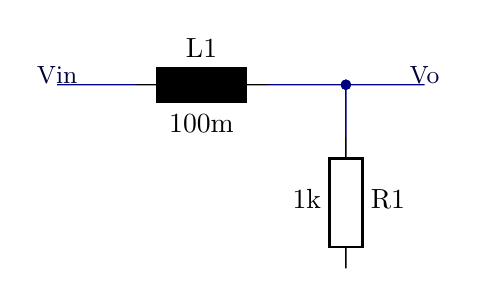
\begin{tikzpicture}[circuit ee IEC, scale=0.6666666667,line width=.5pt]% default: 0.4

\draw [/lt2ti/Net](2.5,-3.0)to[*short,-, color=netcolor] (1.0,-3.0);% wire w3
\draw [/lt2ti/Net](6.5,-3.0)to[*short,*-, color=netcolor] (5.0,-3.0);% wire w4
\draw [/lt2ti/Net](8.0,-3.0)to[*short,-*, color=netcolor] (6.5,-3.0);% wire w5
\draw [/lt2ti/Net](6.5,-4.0)to[*short,-*, color=netcolor] (6.5,-3.0);% wire w6
  \draw (6.5, -4.0) to[*resistor, l^=R1, a_=1k, -, ] (6.5,-6.5){}; %\node [] at (6.0,-3.5) {x}; % component "res" "R1" 
  \draw (2.5, -3.0) to[*inductor, l^=L1, a_=100m, - ] (5.0,-3.0){}; % component "ind" "L1" 
  %\node [] at (2.0,-3.5) {x}; % component "ind" "L1" 
  \node (Vo) [] at (8.0,-3.0) {};% label mark % label "" "Vo" lbl7 
  \node (Votxt) [ netlabelcolor, above= -0.24cm of Vo] {{\pgfkeysvalueof{/lt2ti/netlabel/font}Vo}}; % label "" "Vo" lbl7 
  \node (Vin) [] at (1.0,-3.0) {};% label mark % label "" "Vin" lbl8 
  \node (Vintxt) [ netlabelcolor, above= -0.24cm of Vin] {{\pgfkeysvalueof{/lt2ti/netlabel/font}Vin}}; % label "" "Vin" lbl8 

\end{tikzpicture}

\caption{Figure 2: LR filter circuit}\label{fig:2}
\end{figure}\FloatBarrier

Figure \ref{fig:2} Shows the circuit is comprised of two impedances in series, $R1$ and $L1$ in a potential divider configuration.

The equation  relating the impedance of resistor $R1$ to the frequency is derived as shown by eq.~\ref{eq:3}

\begin{equation}
\begin{split}
    V &= IR\\
    Z &= R = \frac{V}{I}\\
    \therefore Z &= R
\end{split}\label{eq:3}
\end{equation}

The equation relating the impedance of inductor $L1$ to the frequency is derived as shown by eq.~\ref{eq:2}

\begin{equation}
\begin{split}
    V_{L} &= \frac{di}{dt}L\\
    Z &= \frac{V_{L}}{I} = \frac{\frac{d}{dt}L}{I} = \frac{d}{dt}L\\
    \therefore Z &= j\omega L 
\end{split}
\label{eq:2}
\end{equation}

\begin{conditions}
V & IR\\
\frac{d}{dt} & j\omega\\
\end{conditions}

The equation that relates $V_{o}$ to $V_{i}$ with respect to such impedances is given by eq.~\ref{eq:1}

\begin{equation}
    \begin{split}
        \frac{V_{o}}{V_{i}} &= \frac{Z_{2}}{Z_{1}+Z_{2}} \\
        &= \frac{R_{1}}{\frac{d}{dt} L_{1}+R_{1}} \\
    \end{split}
\label{eq:1}
\end{equation}

The fourier frequency response of the circuit is obtained by inserting $j\omega$ in place of $\frac{d}{dt}$ in eq.~\ref{eq:4}

\begin{equation}
    \begin{split}
        \widetilde{\mathcal{F}} \left\{\omega\right\} &= \frac{\widetilde{V}_o\left(\omega\right)}{\widetilde{V}_{in}\left(\omega\right)}\\
          &= \frac{R_{1}}{j\omega L_{1}+R_{1}} \\
          &= \frac{1k\Omega}{j\omega 100mH+1k\Omega} \\
          &= \frac{1000}{j\omega 0.1 + 1000} \\
    \end{split}\label{eq:4}
\end{equation}

$\widetilde{\mathcal{F}}\left(\omega\right)$ can be writen as a transfer function as shown by eq.~\ref{eq:5}

\begin{equation}
    H\left(s\right) = \frac{1000}{0.1\left(s\right) + 1000}
    \label{eq:5}
\end{equation}

Plotting the transfer function in matlabs bode plot function shows the frequency response of the circuit as shown in figure \ref{fig:3}

\begin{figure}[ht!]
\centering
    % This file was created by matlab2tikz.
%
%The latest updates can be retrieved from
%  http://www.mathworks.com/matlabcentral/fileexchange/22022-matlab2tikz-matlab2tikz
%where you can also make suggestions and rate matlab2tikz.
%
\definecolor{mycolor1}{rgb}{0.00000,0.44700,0.74100}%
%
\begin{tikzpicture}

\begin{axis}[%
width=5.303in,
height=1.66in,
at={(0.889in,0.232in)},
scale only axis,
xmode=log,
xmin=100,
xmax=1000000,
xminorticks=true,
ymin=-40.0004342727686,
ymax=0,
ylabel style={font=\color{white!15!black}},
ylabel={Magnitude (dB)},
axis background/.style={fill=white},
title style={font=\bfseries},
title={Bode Diagram}
]
\addplot [color=mycolor1, forget plot]
  table[row sep=crcr]{%
100	-0.000434272768629285\\
218.947676285662	-0.00208142571875669\\
331.528234231942	-0.00477075147159667\\
441.209286319117	-0.00844600301265075\\
550.478980785497	-0.0131404006515297\\
661.943345877439	-0.018987868423693\\
774.263682681121	-0.0259575420087614\\
880.937190447396	-0.0335733326192198\\
993.109181374982	-0.0426231365572747\\
1099.1097009295	-0.0521502353089289\\
1205.26093687084	-0.0626341233849814\\
1321.6641839466	-0.0752074312578728\\
1436.00898465126	-0.0886459278506138\\
1545.92773641949	-0.102570873100753\\
1664.2601764859	-0.118653504907527\\
1775.20801171765	-0.134749729784872\\
1893.5521797563	-0.152991338028293\\
2019.78575681987	-0.173653411723421\\
2154.4346900319	-0.197043251739245\\
2276.97025538168	-0.219521330794869\\
2406.47515001542	-0.244492258570226\\
2543.34576130464	-0.272215746377327\\
2688.00102153763	-0.302974704588593\\
2840.88369018332	-0.337076435850584\\
3002.46170908556	-0.37485368004198\\
3173.22963473497	-0.416665450996113\\
3353.71015200292	-0.462897595779843\\
3544.45567397046	-0.513962998472437\\
3746.05003274901	-0.570301342618976\\
3959.11026646847	-0.632378340730384\\
4184.28850790158	-0.700684336442983\\
4422.27398050588	-0.775732186466129\\
4673.7951079925	-0.858054336557061\\
4939.62174387835	-0.948199019763557\\
5220.56752784699	-1.04672552718515\\
5517.49237612912	-1.15419853225295\\
5831.30511352619	-1.27118148913344\\
6162.96625513299	-1.39822917358004\\
6513.49094627284	-1.53587948858982\\
6883.95206964551	-1.68464471459896\\
7275.48352919622	-1.84500244055315\\
7689.28372075827	-2.01738646297519\\
8201.88949920225	-2.23420630825618\\
8748.6681204799	-2.46841139169483\\
9331.89771573332	-2.72037378069101\\
9954.00828762154	-2.99032608039997\\
10617.5918348299	-3.2783538801952\\
11430.3112911448	-3.62957255285598\\
12305.2400435927	-4.00397978138754\\
13247.1398786611	-4.40100660332678\\
14393.2264471941	-4.87371682509005\\
15638.4675830225	-5.37266961585342\\
17148.8196987055	-5.95586617381813\\
18805.0405512859	-6.5670133742538\\
20812.2156998634	-7.26848046947238\\
23246.9705998564	-8.06465999813501\\
26207.0669648386	-8.95870069070495\\
30093.9003444972	-10.0244376496298\\
35200.3147279666	-11.2680073667815\\
42327.8906557353	-12.7684085990338\\
52810.7971193432	-14.6074457924827\\
69637.4473062821	-16.9455027847075\\
101626.508939299	-20.1819882849523\\
181659.978837533	-25.1983255858367\\
607832.312829721	-35.6768510006815\\
1000000	-40.0004342727686\\
};
\end{axis}
\end{tikzpicture}%
    % This file was created by matlab2tikz.
%
%The latest updates can be retrieved from
%  http://www.mathworks.com/matlabcentral/fileexchange/22022-matlab2tikz-matlab2tikz
%where you can also make suggestions and rate matlab2tikz.
%
\definecolor{mycolor1}{rgb}{0.00000,0.44700,0.74100}%
%
\begin{tikzpicture}

\begin{axis}[%
width=5.303in,
height=1.544in,
at={(0.889in,0.404in)},
scale only axis,
xmode=log,
xmin=100,
xmax=1000000,
xminorticks=true,
xlabel style={font=\color{white!15!black}},
xlabel={Frequency (rad/s)},
ymin=-100,
ymax=0,
ylabel style={font=\color{white!15!black}},
ylabel={Phase (deg)},
axis background/.style={fill=white}
]
\addplot [color=mycolor1, forget plot]
  table[row sep=crcr]{%
100	-0.572938697683483\\
107.654461284232	-0.616790800848705\\
115.894830343983	-0.663998737096861\\
124.765955263085	-0.714819177009232\\
134.316117004601	-0.769528388312366\\
144.597292179202	-0.828423723656115\\
155.665435927107	-0.89182521923594\\
167.580786453079	-0.960077311992777\\
180.408192871936	-1.03355068353132\\
192.435097523032	-1.10243582327779\\
205.263775270926	-1.17590967001985\\
218.947676285666	-1.25427737863302\\
233.543813990646	-1.33786428684678\\
249.11300260678	-1.42701722655684\\
265.720110532454	-1.52210591527894\\
283.434330615128	-1.62352443154175\\
302.329468440578	-1.7316927779424\\
322.484249840847	-1.84705853544169\\
343.982648902288	-1.97009861223668\\
366.914237840248	-2.10132109019342\\
391.374560198041	-2.24126717132471\\
417.46552892532	-2.39051322612191\\
445.295850994262	-2.5496729446558\\
474.981480322851	-2.71939959020092\\
506.646100892133	-2.90038835364977\\
540.421642070586	-3.09337880510022\\
576.448828292587	-3.29915743663557\\
614.877765381008	-3.51856028737438\\
655.868565957134	-3.75247563822874\\
699.592016543535	-4.00184675933943\\
746.230289139115	-4.26767468769374\\
795.977700231511	-4.55102100579367\\
849.041520408869	-4.85301058421723\\
905.642837944531	-5.17483424126608\\
966.017479952276	-5.5177512613521\\
1030.41699495058	-5.88309170005409\\
1099.1097009295	-6.27225838756173\\
1172.38180328661	-6.68672852320007\\
1250.53858729037	-7.12805473157803\\
1333.90569003905	-7.59786542535144\\
1422.83045721436	-8.09786429042008\\
1517.68339028343	-8.62982867650079\\
1618.85969017819	-9.19560663953443\\
1726.78090388436	-9.79711234268261\\
1841.89668079973	-10.4363194805513\\
1964.68664618042	-11.1152523481056\\
2115.07282486879	-11.942467265621\\
2276.97025538168	-12.8273804120148\\
2451.26006203336	-13.7731112921555\\
2638.89081445755	-14.7827363570414\\
2840.88369018327	-15.8592315997175\\
3058.33803237842	-17.0054032260634\\
3292.43733300778	-18.2238055905532\\
3544.45567397046	-19.5166460798951\\
3815.76466127131	-20.8856773646191\\
4107.8408899656	-22.3320784559678\\
4463.23392671036	-24.0523243999599\\
4849.37406733521	-25.8704817729604\\
5268.92142135067	-27.7843937847135\\
5777.79011797049	-30.0184204360201\\
6394.48842855691	-32.5968346709665\\
7142.55928554305	-35.5365477322943\\
8126.61920009201	-39.0994466723111\\
9682.46611930323	-44.0757371068804\\
12650.3372039592	-51.6738846949342\\
14393.2264471941	-55.2095378690207\\
16077.0442167382	-58.1181861493294\\
17793.0438991856	-60.6632563209514\\
19511.483468466	-62.8640121621104\\
21199.5345753606	-64.7463512504026\\
23033.6287314213	-66.5320292016912\\
25026.4009641792	-68.2194358641644\\
27191.5794303603	-69.8084507208634\\
29272.9483504285	-71.139200474058\\
31513.6348486653	-72.3945717309481\\
33925.8338274096	-73.5765587359993\\
36522.6736430817	-74.6875550591854\\
39318.2875570579	-75.7302520543807\\
42327.890655736	-76.7075502688449\\
45567.8626584114	-77.622483822148\\
49055.8370636501	-78.4781571632415\\
52810.7971193432	-79.2776932268564\\
56853.1791387378	-80.0241917980707\\
61204.9837247677	-80.7206968118453\\
65889.8955080006	-81.3701713234992\\
70933.4120498793	-81.9754789546619\\
76362.9826128223	-82.5393707227266\\
81453.717662808	-83.000872418562\\
86883.8263525134	-83.4343626117381\\
92675.9330114683	-83.8414480715644\\
98854.1702191961	-84.2236598020414\\
105444.279352618	-84.5824536201828\\
112473.717836474	-84.9192113806192\\
119971.773543589	-85.2352426991363\\
127969.686821595	-85.5317870523555\\
136500.7806546	-85.8100161519919\\
145600.599502065	-86.0710365103108\\
155307.057393347	-86.3158921288756\\
165660.595894994	-86.5455672557469\\
176704.352608894	-86.7609891672627\\
188484.34090338	-86.9630309396908\\
201049.641626053	-87.1525141836499\\
214452.607597165	-87.3302117204759\\
228749.08173557	-87.496850184875\\
243998.629725958	-87.6531125424178\\
260264.788196897	-87.7996405138609\\
277615.329443679	-87.9370369010414\\
296122.543798806	-88.0658678113147\\
315863.540826787	-88.1866647792611\\
336920.570598025	-88.2999267857794\\
359381.366380464	-88.4061221757628\\
386890.073932801	-88.5193979064433\\
416504.424854525	-88.6246298829198\\
448385.594802114	-88.7223879721031\\
482707.096560317	-88.8132019308138\\
519655.724382768	-88.8975641767222\\
559432.570616944	-88.9759323782962\\
602254.120146203	-89.0487318734598\\
648353.428605466	-89.1163579265961\\
697981.390783064	-89.1791778333487\\
751408.106111699	-89.2375328824053\\
808924.348680602	-89.2917401831172\\
870843.149769087	-89.3420943674399\\
937501.501514519	-89.3888691742858\\
1000000	-89.4270613023165\\
};
\end{axis}
\end{tikzpicture}%
\caption{Figure 3: Frequency Response of the circuit}\label{fig:3}
\end{figure}\FloatBarrier




\subsection{Computing the Impulse Response}\label{subsec:computing_the_impulse_response}
% Determine an expression for the Impulse Response of the circuit using the Frequency Response from Question
% 2.1 as a starting point. [Report: Derivation of Impulse Response with a short comment explaining each step.]

\subsection{Approximating the Impulse Response using LTSpice}\label{subsec:approximating_the_impulse_response_using_ltspice}
% Obtain an approximation for the impulse response of the circuit using a time-domain simulation in LTSpice.
% You need to drive the filter circuit with a Dirac delta function to obtain an output voltage waveform that
% represents the Impulse Response. You cannot use an actual Dirac delta function in LTSpice so you must use
% an approximation.
% Justify the delta approximation you have used and modify the simulation model to test if your approxima-
% tion is influencing the results you obtain - try a few variations on the Delta approximation to see what happens.
% [Report: Figure(s) comparing computed Impulse Response to response obtained using LTSpice and effect of
% different delta approximations, some comments to explain how/why certain delta functions give the correct
% answer but some don’t.]



\subsection{Checking the Frequency Response using LTSpice}\label{subsec:checking_the_frequency_response_using_ltspice}
% Generate Frequency Response plots from your Impulse Response using an FFT. Compare the LTSpice Fre-
% quency Response with your answer to 2.1, how does the Impulse Approximation affect the frequency response
% that you see?

% Include an answer to this question: The frequency response of a circuit is not usually computed using LT-
% Spice by taking an FFT of the Impulse Response, there is another method. What is it? (You don’t need to do
% any further simulations) [Report: Figure(s) comparing computed Frequency Response (2.1) to response obtained
% using LTSpice and comments on: how IR approximation affects results, how FR is usually calculated in software
% such as LTSpice.]

%%%%%%%%%%%%%%%%%%%%%%%%%%%%%%%%%%%%%%%%%%%%%%%%%%%%%%%%%%%%%%%%%%%%%%%%%%%%%%%%%%%%%%%%%
                     % Modelling the filter output using convolution
%%%%%%%%%%%%%%%%%%%%%%%%%%%%%%%%%%%%%%%%%%%%%%%%%%%%%%%%%%%%%%%%%%%%%%%%%%%%%%%%%%%%%%%%%

\section{Modelling the filter output using convolution}\label{sec:modelling_the_filter_output_using_convolution}

\subsection{Deriving the filter output waveform using convolution}\label{subsec:deriving_the_filter_output_waveform_using_convolution}
% Using convolution, compute an expression for the time-domain output waveform of the filter when Vi(t) = S2(t).
% This is the final question for the coursework and is more difficult problem to solve. The process you need
% to follow is exactly the same as in the lecture slides.
% What are the limits of the convolution integral (i.e. where is the product of F (τ ) and S2(t − τ ) non zero)?
% You will need to consider two different sets of limits for different ranges of t. You can start by sketching F (τ )
% S2(t − τ ) on a plot with τ on the horizontal axis to understand these limits.
% As a hint, the only real difference to the lecture example, is that you have a triangle pulse rather than a
% step input. Other than the obvious difference in function shape / different equation for Vin, the limits will be
% different (a step goes on to infinity, and also this pulse doesn’t start at t = 0 like the step in the lecture example).
% [Report: Derivation of time-domain output waveform. Even if you can’t quite get the correct answer for the
% final part, there are marks for attempting this.

\subsection{Comparing the convolution answer to LTSpice}\label{subsec:comparing_the_convolution_answer_to_ltspice}
% Use LTSpice to find Vo when Vi = S2(t). Compare your answer to 3.1 with this.
% [Report: Figure comparing your answer to the time-domain waveform obtained as part of solution to 3.1.


%%%%%%%%%%%%%%%%%%%%%%%%%%%%%%%%%%%%%%%%%%%%%%%%%%%%%%%%%%%%%%%%%%%%%%%%%%%%%%%%%%%%%%%%%
                                    % References
%%%%%%%%%%%%%%%%%%%%%%%%%%%%%%%%%%%%%%%%%%%%%%%%%%%%%%%%%%%%%%%%%%%%%%%%%%%%%%%%%%%%%%%%%

\addcontentsline{toc}{section}{References}
\bibliographystyle{IEEEtranN}
\bibliography{biblist}

%%%%%%%%%%%%%%%%%%%%%%%%%%%%%%%%%%%%%%%%%%%%%%%%%%%%%%%%%%%%%%%%%%%%%%%%%%%%%%%%%%%%%%%%%
                                    % Appendix
%%%%%%%%%%%%%%%%%%%%%%%%%%%%%%%%%%%%%%%%%%%%%%%%%%%%%%%%%%%%%%%%%%%%%%%%%%%%%%%%%%%%%%%%%
\pagebreak
% \appendix
% \section*{Appendices}\addcontentsline{toc}{section}{Appendices}\label{appendix:main}
% \renewcommand{\thesubsection}{\Alph{subsection}}

% \subsection{Matlab Code}

% \subsection{LTSpice Code}

%%%%%%%%%%%%%%%%%%%%%%%%%%%%%%%%%%%%%%%%%%%%%%%%%%%%%%%%%%%%%%%%%%%%%%%%%%%%%%%%%%%%%%%%%
\end{document}


